% Options for packages loaded elsewhere
\PassOptionsToPackage{unicode}{hyperref}
\PassOptionsToPackage{hyphens}{url}
%
\documentclass[
]{article}
\usepackage{amsmath,amssymb}
\usepackage{lmodern}
\usepackage{iftex}
\ifPDFTeX
  \usepackage[T1]{fontenc}
  \usepackage[utf8]{inputenc}
  \usepackage{textcomp} % provide euro and other symbols
\else % if luatex or xetex
  \usepackage{unicode-math}
  \defaultfontfeatures{Scale=MatchLowercase}
  \defaultfontfeatures[\rmfamily]{Ligatures=TeX,Scale=1}
\fi
% Use upquote if available, for straight quotes in verbatim environments
\IfFileExists{upquote.sty}{\usepackage{upquote}}{}
\IfFileExists{microtype.sty}{% use microtype if available
  \usepackage[]{microtype}
  \UseMicrotypeSet[protrusion]{basicmath} % disable protrusion for tt fonts
}{}
\makeatletter
\@ifundefined{KOMAClassName}{% if non-KOMA class
  \IfFileExists{parskip.sty}{%
    \usepackage{parskip}
  }{% else
    \setlength{\parindent}{0pt}
    \setlength{\parskip}{6pt plus 2pt minus 1pt}}
}{% if KOMA class
  \KOMAoptions{parskip=half}}
\makeatother
\usepackage{xcolor}
\IfFileExists{xurl.sty}{\usepackage{xurl}}{} % add URL line breaks if available
\IfFileExists{bookmark.sty}{\usepackage{bookmark}}{\usepackage{hyperref}}
\hypersetup{
  pdftitle={Mini\_project-1`},
  pdfauthor={Susmitha Chereddy - schereddy2371@floridapoly.edu},
  hidelinks,
  pdfcreator={LaTeX via pandoc}}
\urlstyle{same} % disable monospaced font for URLs
\usepackage[margin=1in]{geometry}
\usepackage{color}
\usepackage{fancyvrb}
\newcommand{\VerbBar}{|}
\newcommand{\VERB}{\Verb[commandchars=\\\{\}]}
\DefineVerbatimEnvironment{Highlighting}{Verbatim}{commandchars=\\\{\}}
% Add ',fontsize=\small' for more characters per line
\usepackage{framed}
\definecolor{shadecolor}{RGB}{248,248,248}
\newenvironment{Shaded}{\begin{snugshade}}{\end{snugshade}}
\newcommand{\AlertTok}[1]{\textcolor[rgb]{0.94,0.16,0.16}{#1}}
\newcommand{\AnnotationTok}[1]{\textcolor[rgb]{0.56,0.35,0.01}{\textbf{\textit{#1}}}}
\newcommand{\AttributeTok}[1]{\textcolor[rgb]{0.77,0.63,0.00}{#1}}
\newcommand{\BaseNTok}[1]{\textcolor[rgb]{0.00,0.00,0.81}{#1}}
\newcommand{\BuiltInTok}[1]{#1}
\newcommand{\CharTok}[1]{\textcolor[rgb]{0.31,0.60,0.02}{#1}}
\newcommand{\CommentTok}[1]{\textcolor[rgb]{0.56,0.35,0.01}{\textit{#1}}}
\newcommand{\CommentVarTok}[1]{\textcolor[rgb]{0.56,0.35,0.01}{\textbf{\textit{#1}}}}
\newcommand{\ConstantTok}[1]{\textcolor[rgb]{0.00,0.00,0.00}{#1}}
\newcommand{\ControlFlowTok}[1]{\textcolor[rgb]{0.13,0.29,0.53}{\textbf{#1}}}
\newcommand{\DataTypeTok}[1]{\textcolor[rgb]{0.13,0.29,0.53}{#1}}
\newcommand{\DecValTok}[1]{\textcolor[rgb]{0.00,0.00,0.81}{#1}}
\newcommand{\DocumentationTok}[1]{\textcolor[rgb]{0.56,0.35,0.01}{\textbf{\textit{#1}}}}
\newcommand{\ErrorTok}[1]{\textcolor[rgb]{0.64,0.00,0.00}{\textbf{#1}}}
\newcommand{\ExtensionTok}[1]{#1}
\newcommand{\FloatTok}[1]{\textcolor[rgb]{0.00,0.00,0.81}{#1}}
\newcommand{\FunctionTok}[1]{\textcolor[rgb]{0.00,0.00,0.00}{#1}}
\newcommand{\ImportTok}[1]{#1}
\newcommand{\InformationTok}[1]{\textcolor[rgb]{0.56,0.35,0.01}{\textbf{\textit{#1}}}}
\newcommand{\KeywordTok}[1]{\textcolor[rgb]{0.13,0.29,0.53}{\textbf{#1}}}
\newcommand{\NormalTok}[1]{#1}
\newcommand{\OperatorTok}[1]{\textcolor[rgb]{0.81,0.36,0.00}{\textbf{#1}}}
\newcommand{\OtherTok}[1]{\textcolor[rgb]{0.56,0.35,0.01}{#1}}
\newcommand{\PreprocessorTok}[1]{\textcolor[rgb]{0.56,0.35,0.01}{\textit{#1}}}
\newcommand{\RegionMarkerTok}[1]{#1}
\newcommand{\SpecialCharTok}[1]{\textcolor[rgb]{0.00,0.00,0.00}{#1}}
\newcommand{\SpecialStringTok}[1]{\textcolor[rgb]{0.31,0.60,0.02}{#1}}
\newcommand{\StringTok}[1]{\textcolor[rgb]{0.31,0.60,0.02}{#1}}
\newcommand{\VariableTok}[1]{\textcolor[rgb]{0.00,0.00,0.00}{#1}}
\newcommand{\VerbatimStringTok}[1]{\textcolor[rgb]{0.31,0.60,0.02}{#1}}
\newcommand{\WarningTok}[1]{\textcolor[rgb]{0.56,0.35,0.01}{\textbf{\textit{#1}}}}
\usepackage{graphicx}
\makeatletter
\def\maxwidth{\ifdim\Gin@nat@width>\linewidth\linewidth\else\Gin@nat@width\fi}
\def\maxheight{\ifdim\Gin@nat@height>\textheight\textheight\else\Gin@nat@height\fi}
\makeatother
% Scale images if necessary, so that they will not overflow the page
% margins by default, and it is still possible to overwrite the defaults
% using explicit options in \includegraphics[width, height, ...]{}
\setkeys{Gin}{width=\maxwidth,height=\maxheight,keepaspectratio}
% Set default figure placement to htbp
\makeatletter
\def\fps@figure{htbp}
\makeatother
\setlength{\emergencystretch}{3em} % prevent overfull lines
\providecommand{\tightlist}{%
  \setlength{\itemsep}{0pt}\setlength{\parskip}{0pt}}
\setcounter{secnumdepth}{-\maxdimen} % remove section numbering
\ifLuaTeX
  \usepackage{selnolig}  % disable illegal ligatures
\fi

\title{Mini\_project-1`}
\author{Susmitha Chereddy - \texttt{schereddy2371@floridapoly.edu}}
\date{}

\begin{document}
\maketitle

This is an \href{http://rmarkdown.rstudio.com}{R Markdown} Notebook.
When you execute code within the notebook, the results appear beneath
the code.

Try executing this chunk by clicking the \emph{Run} button within the
chunk or by placing your cursor inside it and pressing
\emph{Ctrl+Shift+Enter}.

\begin{Shaded}
\begin{Highlighting}[]
\FunctionTok{library}\NormalTok{(tidyverse)}
\end{Highlighting}
\end{Shaded}

Loading Us Birth data from 2000 to 2014

\begin{Shaded}
\begin{Highlighting}[]
\NormalTok{birth\_data}\OtherTok{\textless{}{-}}\FunctionTok{read\_csv}\NormalTok{(}\StringTok{"C:/Susmitha Chereddy/Data\_visualization/Mini\_project\_1\_chereddy/data/birth\_data.csv"}\NormalTok{)}
\end{Highlighting}
\end{Shaded}

\begin{verbatim}
## Rows: 5479 Columns: 6
## -- Column specification --------------------------------------------------------
## Delimiter: ","
## chr  (1): day_of_week
## dbl  (4): year, month, date_of_month, births
## date (1): date
## 
## i Use `spec()` to retrieve the full column specification for this data.
## i Specify the column types or set `show_col_types = FALSE` to quiet this message.
\end{verbatim}

\begin{Shaded}
\begin{Highlighting}[]
\FunctionTok{str}\NormalTok{(birth\_data)}
\end{Highlighting}
\end{Shaded}

\begin{verbatim}
## spec_tbl_df [5,479 x 6] (S3: spec_tbl_df/tbl_df/tbl/data.frame)
##  $ year         : num [1:5479] 2000 2000 2000 2000 2000 2000 2000 2000 2000 2000 ...
##  $ month        : num [1:5479] 1 1 1 1 1 1 1 1 1 1 ...
##  $ date_of_month: num [1:5479] 1 2 3 4 5 6 7 8 9 10 ...
##  $ date         : Date[1:5479], format: "2000-01-01" "2000-01-02" ...
##  $ day_of_week  : chr [1:5479] "Sat" "Sun" "Mon" "Tues" ...
##  $ births       : num [1:5479] 9083 8006 11363 13032 12558 ...
##  - attr(*, "spec")=
##   .. cols(
##   ..   year = col_double(),
##   ..   month = col_double(),
##   ..   date_of_month = col_double(),
##   ..   date = col_date(format = ""),
##   ..   day_of_week = col_character(),
##   ..   births = col_double()
##   .. )
##  - attr(*, "problems")=<externalptr>
\end{verbatim}

converting year, month , date\_of\_month, day\_of\_week as factor

\begin{Shaded}
\begin{Highlighting}[]
\NormalTok{birth\_data }\OtherTok{\textless{}{-}}\NormalTok{ birth\_data }\SpecialCharTok{\%\textgreater{}\%}
  \FunctionTok{mutate}\NormalTok{(}\AttributeTok{month=}\FunctionTok{as\_factor}\NormalTok{(month)) }\SpecialCharTok{\%\textgreater{}\%}
  \FunctionTok{mutate}\NormalTok{(}\AttributeTok{year=}\FunctionTok{as\_factor}\NormalTok{(year)) }\SpecialCharTok{\%\textgreater{}\%}
  \FunctionTok{mutate}\NormalTok{(}\AttributeTok{day\_of\_week=}\FunctionTok{as\_factor}\NormalTok{(day\_of\_week)) }\SpecialCharTok{\%\textgreater{}\%}
  \FunctionTok{mutate}\NormalTok{(}\AttributeTok{date\_of\_month=}\FunctionTok{as\_factor}\NormalTok{(date\_of\_month))}

\FunctionTok{str}\NormalTok{(birth\_data)}
\end{Highlighting}
\end{Shaded}

\begin{verbatim}
## tibble [5,479 x 6] (S3: tbl_df/tbl/data.frame)
##  $ year         : Factor w/ 15 levels "2000","2001",..: 1 1 1 1 1 1 1 1 1 1 ...
##  $ month        : Factor w/ 12 levels "1","2","3","4",..: 1 1 1 1 1 1 1 1 1 1 ...
##  $ date_of_month: Factor w/ 31 levels "1","2","3","4",..: 1 2 3 4 5 6 7 8 9 10 ...
##  $ date         : Date[1:5479], format: "2000-01-01" "2000-01-02" ...
##  $ day_of_week  : Factor w/ 7 levels "Sat","Sun","Mon",..: 1 2 3 4 5 6 7 1 2 3 ...
##  $ births       : num [1:5479] 9083 8006 11363 13032 12558 ...
\end{verbatim}

Assigning levels to Month and day\_of\_week

\begin{Shaded}
\begin{Highlighting}[]
\FunctionTok{levels}\NormalTok{(birth\_data}\SpecialCharTok{$}\NormalTok{day\_of\_week) }\OtherTok{\textless{}{-}} \FunctionTok{c}\NormalTok{(}\StringTok{"Monday"}\NormalTok{, }\StringTok{"Tuesday"}\NormalTok{, }\StringTok{"Wednesday"}\NormalTok{, }\StringTok{"Thursday"}\NormalTok{, }\StringTok{"Friday"}\NormalTok{, }\StringTok{"Saturday"}\NormalTok{, }\StringTok{"Sunday"}\NormalTok{)}

\FunctionTok{levels}\NormalTok{(birth\_data}\SpecialCharTok{$}\NormalTok{month) }\OtherTok{\textless{}{-}} \FunctionTok{c}\NormalTok{(}\StringTok{"January"}\NormalTok{, }\StringTok{"February"}\NormalTok{, }\StringTok{"March"}\NormalTok{, }\StringTok{"April"}\NormalTok{, }\StringTok{"May"}\NormalTok{, }\StringTok{"June"}\NormalTok{, }\StringTok{"July"}\NormalTok{, }\StringTok{"August"}\NormalTok{, }\StringTok{"September"}\NormalTok{, }\StringTok{"October"}\NormalTok{, }\StringTok{"November"}\NormalTok{, }\StringTok{"December"}\NormalTok{)}

\NormalTok{birth\_data}
\end{Highlighting}
\end{Shaded}

\begin{verbatim}
## # A tibble: 5,479 x 6
##    year  month   date_of_month date       day_of_week births
##    <fct> <fct>   <fct>         <date>     <fct>        <dbl>
##  1 2000  January 1             2000-01-01 Monday        9083
##  2 2000  January 2             2000-01-02 Tuesday       8006
##  3 2000  January 3             2000-01-03 Wednesday    11363
##  4 2000  January 4             2000-01-04 Thursday     13032
##  5 2000  January 5             2000-01-05 Friday       12558
##  6 2000  January 6             2000-01-06 Saturday     12466
##  7 2000  January 7             2000-01-07 Sunday       12516
##  8 2000  January 8             2000-01-08 Monday        8934
##  9 2000  January 9             2000-01-09 Tuesday       7949
## 10 2000  January 10            2000-01-10 Wednesday    11668
## # ... with 5,469 more rows
\end{verbatim}

\begin{Shaded}
\begin{Highlighting}[]
\NormalTok{birth\_data\_by\_year }\OtherTok{\textless{}{-}}\NormalTok{ birth\_data }\SpecialCharTok{\%\textgreater{}\%} 
  \FunctionTok{group\_by}\NormalTok{(year) }\SpecialCharTok{\%\textgreater{}\%} 
  \FunctionTok{summarize}\NormalTok{(}\AttributeTok{total\_by\_year =} \FunctionTok{sum}\NormalTok{(births))}

\NormalTok{birth\_data\_by\_year}
\end{Highlighting}
\end{Shaded}

\begin{verbatim}
## # A tibble: 15 x 2
##    year  total_by_year
##    <fct>         <dbl>
##  1 2000        4149598
##  2 2001        4110963
##  3 2002        4099313
##  4 2003        4163060
##  5 2004        4186863
##  6 2005        4211941
##  7 2006        4335154
##  8 2007        4380784
##  9 2008        4310737
## 10 2009        4190991
## 11 2010        4055975
## 12 2011        4006908
## 13 2012        4000868
## 14 2013        3973337
## 15 2014        4010532
\end{verbatim}

\begin{Shaded}
\begin{Highlighting}[]
\CommentTok{\#ggplot(data= birth\_data\_by\_year,aes(x=year, y=total\_by\_year),color=purple)+geom\_col()}
\FunctionTok{ggplot}\NormalTok{(}\AttributeTok{data=}\NormalTok{ birth\_data\_by\_year,}\FunctionTok{aes}\NormalTok{(}\AttributeTok{x=}\NormalTok{year, }\AttributeTok{y=}\NormalTok{total\_by\_year))}\SpecialCharTok{+}
  \FunctionTok{geom\_bar}\NormalTok{(}\AttributeTok{stat=}\StringTok{"identity"}\NormalTok{,}\AttributeTok{fill=}\StringTok{"light blue"}\NormalTok{,}\AttributeTok{color=}\StringTok{"purple"}\NormalTok{)}\SpecialCharTok{+}
  \FunctionTok{scale\_y\_continuous}\NormalTok{(}\AttributeTok{limits =} \FunctionTok{c}\NormalTok{(}\DecValTok{0}\NormalTok{, }\DecValTok{4500000}\NormalTok{))}\SpecialCharTok{+}
  \FunctionTok{labs}\NormalTok{(}\AttributeTok{title =} \StringTok{"US Births by Year from 2000 to 2014"}\NormalTok{,}
       \AttributeTok{caption=}\StringTok{"US Births from 2000{-}2014"}\NormalTok{)}\SpecialCharTok{+}
  \FunctionTok{xlab}\NormalTok{(}\StringTok{"Year of Birth"}\NormalTok{) }\SpecialCharTok{+}
  \FunctionTok{ylab}\NormalTok{(}\StringTok{"Total Births"}\NormalTok{)}
\end{Highlighting}
\end{Shaded}

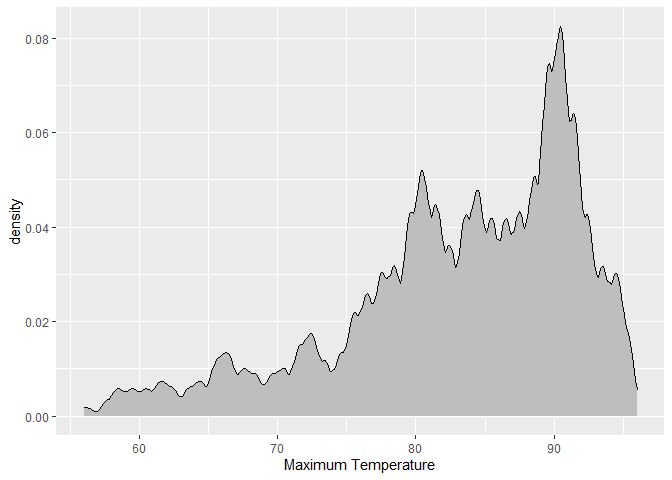
\includegraphics{Birth_data_report_chereddy_files/figure-latex/unnamed-chunk-6-1.pdf}

\begin{Shaded}
\begin{Highlighting}[]
\NormalTok{birth\_data\_by\_month }\OtherTok{\textless{}{-}}\NormalTok{ birth\_data }\SpecialCharTok{\%\textgreater{}\%} 
  \FunctionTok{group\_by}\NormalTok{(month) }\SpecialCharTok{\%\textgreater{}\%} 
  \FunctionTok{summarize}\NormalTok{(}\AttributeTok{total\_by\_month =} \FunctionTok{sum}\NormalTok{(births))}

\NormalTok{birth\_data\_by\_month}
\end{Highlighting}
\end{Shaded}

\begin{verbatim}
## # A tibble: 12 x 2
##    month     total_by_month
##    <fct>              <dbl>
##  1 January          5072588
##  2 February         4725693
##  3 March            5172961
##  4 April            4960750
##  5 May              5195445
##  6 June             5163360
##  7 July             5450418
##  8 August           5540170
##  9 September        5399592
## 10 October          5302865
## 11 November         5008750
## 12 December         5194432
\end{verbatim}

\begin{Shaded}
\begin{Highlighting}[]
\FunctionTok{ggplot}\NormalTok{(}\AttributeTok{data=}\NormalTok{ birth\_data\_by\_month,}\FunctionTok{aes}\NormalTok{(}\AttributeTok{x=}\NormalTok{month, }\AttributeTok{y=}\NormalTok{total\_by\_month))}\SpecialCharTok{+}
  \FunctionTok{geom\_bar}\NormalTok{(}\AttributeTok{stat=}\StringTok{"identity"}\NormalTok{,}\AttributeTok{fill=}\StringTok{"light blue"}\NormalTok{,}\AttributeTok{color=}\StringTok{"purple"}\NormalTok{)}\SpecialCharTok{+}
  \FunctionTok{scale\_y\_continuous}\NormalTok{(}\AttributeTok{limits =} \FunctionTok{c}\NormalTok{(}\DecValTok{0}\NormalTok{, }\DecValTok{6000000}\NormalTok{))}\SpecialCharTok{+}
  \FunctionTok{labs}\NormalTok{(}\AttributeTok{title =} \StringTok{"US Births by month from 2000 to 2014"}\NormalTok{,}
       \AttributeTok{caption=}\StringTok{"US Births from 2000{-}2014"}\NormalTok{)}\SpecialCharTok{+}
  \FunctionTok{xlab}\NormalTok{(}\StringTok{"Month of Birth"}\NormalTok{) }\SpecialCharTok{+}
  \FunctionTok{ylab}\NormalTok{(}\StringTok{"Total Births"}\NormalTok{)}
\end{Highlighting}
\end{Shaded}

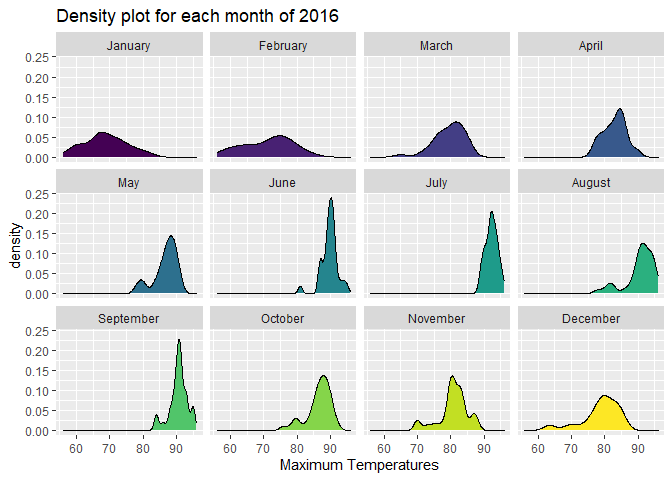
\includegraphics{Birth_data_report_chereddy_files/figure-latex/unnamed-chunk-8-1.pdf}

\begin{Shaded}
\begin{Highlighting}[]
\NormalTok{birth\_data\_by\_day }\OtherTok{\textless{}{-}}\NormalTok{ birth\_data }\SpecialCharTok{\%\textgreater{}\%} 
  \FunctionTok{group\_by}\NormalTok{(day\_of\_week) }\SpecialCharTok{\%\textgreater{}\%} 
  \FunctionTok{summarize}\NormalTok{(}\AttributeTok{total\_by\_day =} \FunctionTok{sum}\NormalTok{(births))}

\NormalTok{birth\_data\_by\_day}
\end{Highlighting}
\end{Shaded}

\begin{verbatim}
## # A tibble: 7 x 2
##   day_of_week total_by_day
##   <fct>              <dbl>
## 1 Monday           6704495
## 2 Tuesday          5886889
## 3 Wednesday        9316001
## 4 Thursday        10274874
## 5 Friday          10109130
## 6 Saturday        10045436
## 7 Sunday           9850199
\end{verbatim}

\begin{Shaded}
\begin{Highlighting}[]
\FunctionTok{ggplot}\NormalTok{(}\AttributeTok{data=}\NormalTok{ birth\_data\_by\_day,}\FunctionTok{aes}\NormalTok{(}\AttributeTok{x=}\NormalTok{day\_of\_week, }\AttributeTok{y=}\NormalTok{total\_by\_day))}\SpecialCharTok{+}
  \FunctionTok{geom\_bar}\NormalTok{(}\AttributeTok{stat=}\StringTok{"identity"}\NormalTok{,}\AttributeTok{fill=}\StringTok{"light blue"}\NormalTok{,}\AttributeTok{color=}\StringTok{"purple"}\NormalTok{)}\SpecialCharTok{+}
  \FunctionTok{scale\_y\_continuous}\NormalTok{(}\AttributeTok{limits =} \FunctionTok{c}\NormalTok{(}\DecValTok{0}\NormalTok{, }\DecValTok{11000000}\NormalTok{))}\SpecialCharTok{+}
  \FunctionTok{labs}\NormalTok{(}\AttributeTok{title =} \StringTok{"US Births by day of week from 2000 to 2014"}\NormalTok{,}
       \AttributeTok{caption=}\StringTok{"US Births from 2000{-}2014"}\NormalTok{)}\SpecialCharTok{+}
  \FunctionTok{xlab}\NormalTok{(}\StringTok{"day in week of Birth"}\NormalTok{) }\SpecialCharTok{+}
  \FunctionTok{ylab}\NormalTok{(}\StringTok{"Total Births"}\NormalTok{)}
\end{Highlighting}
\end{Shaded}

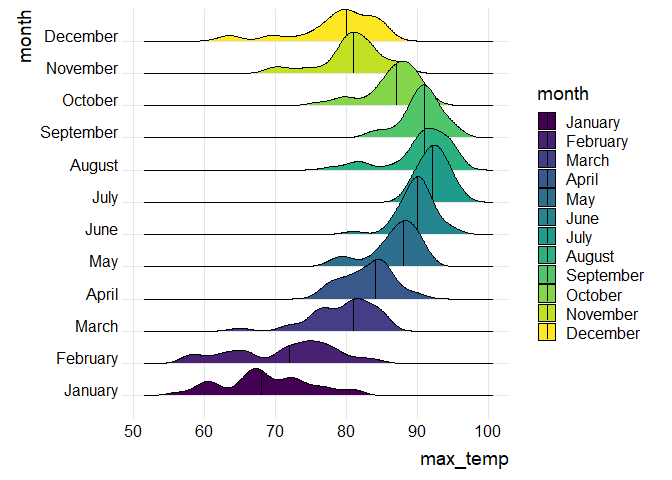
\includegraphics{Birth_data_report_chereddy_files/figure-latex/unnamed-chunk-10-1.pdf}

\begin{Shaded}
\begin{Highlighting}[]
\NormalTok{birth\_data\_by\_date }\OtherTok{\textless{}{-}}\NormalTok{ birth\_data }\SpecialCharTok{\%\textgreater{}\%} 
  \FunctionTok{group\_by}\NormalTok{(date\_of\_month) }\SpecialCharTok{\%\textgreater{}\%} 
  \FunctionTok{summarize}\NormalTok{(}\AttributeTok{total\_by\_date =} \FunctionTok{sum}\NormalTok{(births))}

\NormalTok{birth\_data\_by\_date}
\end{Highlighting}
\end{Shaded}

\begin{verbatim}
## # A tibble: 31 x 2
##    date_of_month total_by_date
##    <fct>                 <dbl>
##  1 1                   2003627
##  2 2                   2030447
##  3 3                   2042441
##  4 4                   2004785
##  5 5                   2036185
##  6 6                   2037729
##  7 7                   2063416
##  8 8                   2061652
##  9 9                   2044600
## 10 10                  2066154
## # ... with 21 more rows
\end{verbatim}

\begin{Shaded}
\begin{Highlighting}[]
\FunctionTok{ggplot}\NormalTok{(}\AttributeTok{data=}\NormalTok{ birth\_data\_by\_date,}\FunctionTok{aes}\NormalTok{(}\AttributeTok{x=}\NormalTok{date\_of\_month, }\AttributeTok{y=}\NormalTok{total\_by\_date))}\SpecialCharTok{+}
  \FunctionTok{geom\_bar}\NormalTok{(}\AttributeTok{stat=}\StringTok{"identity"}\NormalTok{,}\AttributeTok{fill=}\StringTok{"light blue"}\NormalTok{,}\AttributeTok{color=}\StringTok{"purple"}\NormalTok{)}\SpecialCharTok{+}
  \FunctionTok{scale\_y\_continuous}\NormalTok{(}\AttributeTok{limits =} \FunctionTok{c}\NormalTok{(}\DecValTok{0}\NormalTok{, }\DecValTok{2500000}\NormalTok{))}\SpecialCharTok{+}
  \FunctionTok{labs}\NormalTok{(}\AttributeTok{title =} \StringTok{"US Births by date of month from 2000 to 2014"}\NormalTok{,}
       \AttributeTok{caption=}\StringTok{"US Births from 2000{-}2014"}\NormalTok{)}\SpecialCharTok{+}
  \FunctionTok{xlab}\NormalTok{(}\StringTok{"date in month of Birth"}\NormalTok{) }\SpecialCharTok{+}
  \FunctionTok{ylab}\NormalTok{(}\StringTok{"Total Births"}\NormalTok{)}
\end{Highlighting}
\end{Shaded}

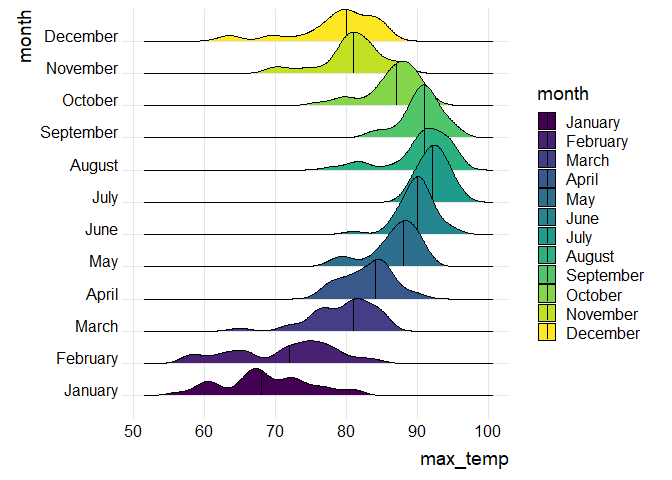
\includegraphics{Birth_data_report_chereddy_files/figure-latex/unnamed-chunk-12-1.pdf}

Let us look at some density plots: This density plots give us a
distribution of births very similar to a histogram

\begin{Shaded}
\begin{Highlighting}[]
\FunctionTok{ggplot}\NormalTok{(}\AttributeTok{data=}\NormalTok{birth\_data, }\FunctionTok{aes}\NormalTok{(births)) }\SpecialCharTok{+} 
  \FunctionTok{geom\_density}\NormalTok{()}\SpecialCharTok{+}
  \FunctionTok{labs}\NormalTok{(}\AttributeTok{title =} \StringTok{"US Births by Year from 2000 to 2014"}\NormalTok{,}
       \AttributeTok{caption=}\StringTok{" 2000{-}2014"}\NormalTok{)}\SpecialCharTok{+}
  \FunctionTok{xlab}\NormalTok{(}\StringTok{"Birth"}\NormalTok{) }\SpecialCharTok{+}
  \FunctionTok{ylab}\NormalTok{(}\StringTok{"Total density"}\NormalTok{)}
\end{Highlighting}
\end{Shaded}

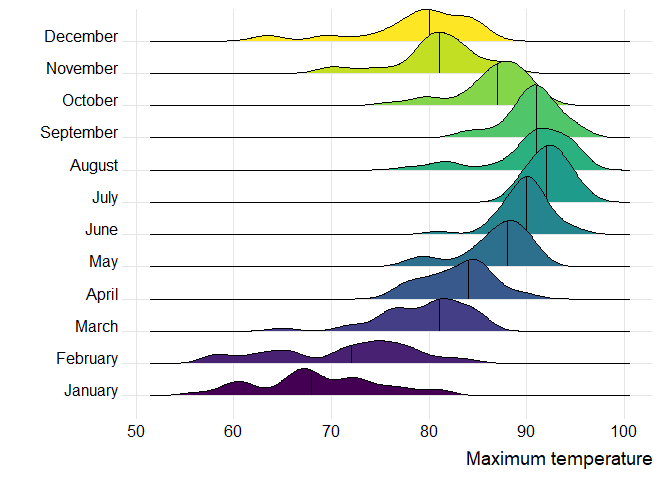
\includegraphics{Birth_data_report_chereddy_files/figure-latex/unnamed-chunk-13-1.pdf}

Let us look at some density plots: This density plots give us a
distribution of births very similar to a histogram

\begin{Shaded}
\begin{Highlighting}[]
\FunctionTok{ggplot}\NormalTok{(}\AttributeTok{data=}\NormalTok{birth\_data, }\FunctionTok{aes}\NormalTok{(}\AttributeTok{x=}\NormalTok{births,}\AttributeTok{color=}\NormalTok{month)) }\SpecialCharTok{+} 
  \FunctionTok{geom\_density}\NormalTok{()}\SpecialCharTok{+}
  \FunctionTok{labs}\NormalTok{(}\AttributeTok{title =} \StringTok{"US Births by Year from 2000 to 2014"}\NormalTok{,}
       \AttributeTok{caption=}\StringTok{" 2000{-}2014"}\NormalTok{)}\SpecialCharTok{+}
  \FunctionTok{xlab}\NormalTok{(}\StringTok{"Birth"}\NormalTok{) }\SpecialCharTok{+}
  \FunctionTok{ylab}\NormalTok{(}\StringTok{"Density"}\NormalTok{)}
\end{Highlighting}
\end{Shaded}

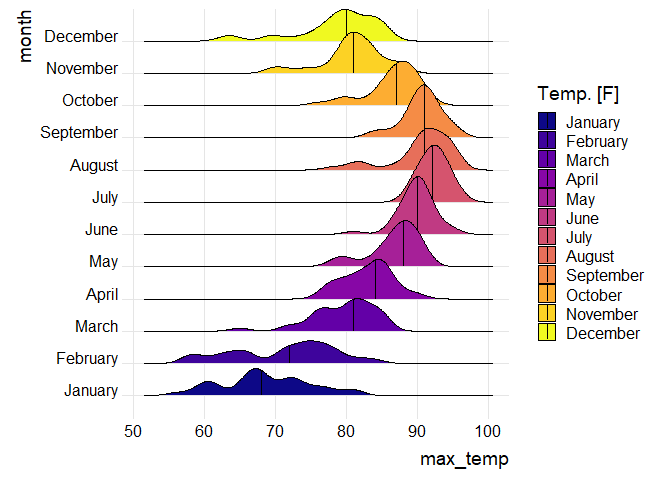
\includegraphics{Birth_data_report_chereddy_files/figure-latex/unnamed-chunk-14-1.pdf}
Let us answer the same question about low birth rate on weekends with a
density plot. here we can see that mean on sat and sun is much less
compared to other days.

\begin{Shaded}
\begin{Highlighting}[]
\FunctionTok{ggplot}\NormalTok{(}\AttributeTok{data=}\NormalTok{birth\_data, }\FunctionTok{aes}\NormalTok{(births,}\AttributeTok{color=}\NormalTok{year)) }\SpecialCharTok{+} 
  \FunctionTok{geom\_density}\NormalTok{()}\SpecialCharTok{+}
  \FunctionTok{facet\_wrap}\NormalTok{(}\SpecialCharTok{\textasciitilde{}}\NormalTok{day\_of\_week)}\SpecialCharTok{+}
  \FunctionTok{labs}\NormalTok{(}\AttributeTok{title =} \StringTok{"Distribution of US Births by day of week "}\NormalTok{,}
       \AttributeTok{caption=}\StringTok{"US Births from 2000{-}2014"}\NormalTok{)}\SpecialCharTok{+}
  \FunctionTok{xlab}\NormalTok{(}\StringTok{"Births"}\NormalTok{) }\SpecialCharTok{+}
  \FunctionTok{ylab}\NormalTok{(}\StringTok{"Density"}\NormalTok{)}
\end{Highlighting}
\end{Shaded}

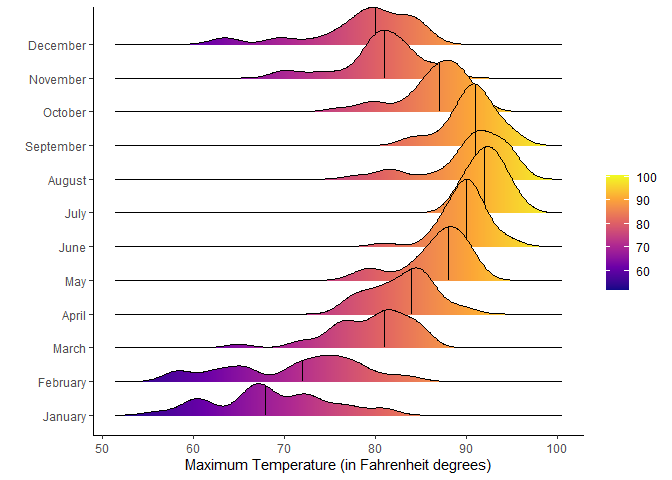
\includegraphics{Birth_data_report_chereddy_files/figure-latex/unnamed-chunk-15-1.pdf}

\begin{Shaded}
\begin{Highlighting}[]
\FunctionTok{ggplot}\NormalTok{(}\AttributeTok{data=}\NormalTok{birth\_data, }\FunctionTok{aes}\NormalTok{(births,}\AttributeTok{color=}\NormalTok{year)) }\SpecialCharTok{+} 
  \FunctionTok{geom\_density}\NormalTok{()}\SpecialCharTok{+}
  \FunctionTok{facet\_wrap}\NormalTok{(month}\SpecialCharTok{\textasciitilde{}}\NormalTok{day\_of\_week)}\SpecialCharTok{+}
  \FunctionTok{labs}\NormalTok{(}\AttributeTok{title =} \StringTok{"US Births by Year from 2000 to 2014{-} Facet wrap"}\NormalTok{,}
       \AttributeTok{caption=}\StringTok{" 2000{-}2014"}\NormalTok{)}\SpecialCharTok{+}
  \FunctionTok{xlab}\NormalTok{(}\StringTok{"Birth"}\NormalTok{) }\SpecialCharTok{+}
  \FunctionTok{ylab}\NormalTok{(}\StringTok{"Density"}\NormalTok{)}
\end{Highlighting}
\end{Shaded}

\includegraphics{Birth_data_report_chereddy_files/figure-latex/unnamed-chunk-16-1.pdf}

Now let's try to more clearly separate weekends and weekdays

\begin{Shaded}
\begin{Highlighting}[]
\NormalTok{birth\_data }\OtherTok{\textless{}{-}}\NormalTok{ birth\_data }\SpecialCharTok{\%\textgreater{}\%}
  \FunctionTok{mutate}\NormalTok{(}\AttributeTok{is\_weekend =} \FunctionTok{if\_else}\NormalTok{(day\_of\_week }\SpecialCharTok{==} \StringTok{"Sat"} \SpecialCharTok{|}\NormalTok{ day\_of\_week }\SpecialCharTok{==} \StringTok{"Sun"}\NormalTok{,}\StringTok{"Yes"}\NormalTok{,}\StringTok{"No"}\NormalTok{))}
\NormalTok{birth\_data}
\end{Highlighting}
\end{Shaded}

\begin{verbatim}
## # A tibble: 5,479 x 7
##    year  month   date_of_month date       day_of_week births is_weekend
##    <fct> <fct>   <fct>         <date>     <fct>        <dbl> <chr>     
##  1 2000  January 1             2000-01-01 Monday        9083 No        
##  2 2000  January 2             2000-01-02 Tuesday       8006 No        
##  3 2000  January 3             2000-01-03 Wednesday    11363 No        
##  4 2000  January 4             2000-01-04 Thursday     13032 No        
##  5 2000  January 5             2000-01-05 Friday       12558 No        
##  6 2000  January 6             2000-01-06 Saturday     12466 No        
##  7 2000  January 7             2000-01-07 Sunday       12516 No        
##  8 2000  January 8             2000-01-08 Monday        8934 No        
##  9 2000  January 9             2000-01-09 Tuesday       7949 No        
## 10 2000  January 10            2000-01-10 Wednesday    11668 No        
## # ... with 5,469 more rows
\end{verbatim}

\begin{Shaded}
\begin{Highlighting}[]
\NormalTok{birth\_data\_weekend }\OtherTok{\textless{}{-}}\NormalTok{ birth\_data }\SpecialCharTok{\%\textgreater{}\%} 
  \FunctionTok{group\_by}\NormalTok{(is\_weekend) }\SpecialCharTok{\%\textgreater{}\%} 
  \FunctionTok{summarize}\NormalTok{(}\AttributeTok{mean =} \FunctionTok{mean}\NormalTok{(births))}

\NormalTok{birth\_data\_weekend}
\end{Highlighting}
\end{Shaded}

\begin{verbatim}
## # A tibble: 1 x 2
##   is_weekend   mean
##   <chr>       <dbl>
## 1 No         11350.
\end{verbatim}

From this ,we can clearly say that Number of births on the weekend is
much higher than the number of births during the week days.

Now let's plot some time series plots to see if it can shed more light
on distribution of Births data.

\begin{Shaded}
\begin{Highlighting}[]
\NormalTok{birth\_data\_date }\OtherTok{\textless{}{-}}\NormalTok{ birth\_data }\SpecialCharTok{\%\textgreater{}\%} \FunctionTok{arrange}\NormalTok{(date)}
\NormalTok{birth\_data\_date}
\end{Highlighting}
\end{Shaded}

\begin{verbatim}
## # A tibble: 5,479 x 7
##    year  month   date_of_month date       day_of_week births is_weekend
##    <fct> <fct>   <fct>         <date>     <fct>        <dbl> <chr>     
##  1 2000  January 1             2000-01-01 Monday        9083 No        
##  2 2000  January 2             2000-01-02 Tuesday       8006 No        
##  3 2000  January 3             2000-01-03 Wednesday    11363 No        
##  4 2000  January 4             2000-01-04 Thursday     13032 No        
##  5 2000  January 5             2000-01-05 Friday       12558 No        
##  6 2000  January 6             2000-01-06 Saturday     12466 No        
##  7 2000  January 7             2000-01-07 Sunday       12516 No        
##  8 2000  January 8             2000-01-08 Monday        8934 No        
##  9 2000  January 9             2000-01-09 Tuesday       7949 No        
## 10 2000  January 10            2000-01-10 Wednesday    11668 No        
## # ... with 5,469 more rows
\end{verbatim}

\#REPORT

This projects aims at summaraizing and analyzing the birth data in US
from 2000 - 2014. reports starts with a preliminary understanding of the
data with some exploratory analysis and then proceeds towards developing
a story about the trend of births in weekdays over weekends. we have
used barcharts, density plot and facetwraps to demonstrate the same.
In-order to provide additional support, we have provide some mean
analysis as well to support our assumption.

\textbf{At the end, all our charts and analysis point out to the
direction that our hypotheiss that number of births on weekend are low
is infact true.}

\textbf{What were the original charts you planned to create for this
assignments?}

I wanted to use some scatter plots, pie charts and timeseries on the
data since the data is mostly about date,days, year and months..
however, i quickly realized for the questions i am trying to answer,
barcharts/histograms are the best option and I went ahead with a
barchart to show how the births on weekend are more than weekdays.

\begin{Shaded}
\begin{Highlighting}[]
\FunctionTok{ggplot}\NormalTok{(birth\_data,}\FunctionTok{aes}\NormalTok{(}\AttributeTok{x=}\NormalTok{date,}\AttributeTok{y=}\NormalTok{births))}\SpecialCharTok{+}
  \FunctionTok{geom\_line}\NormalTok{(}\AttributeTok{color =} \StringTok{"purple"}\NormalTok{) }\SpecialCharTok{+} 
    \FunctionTok{scale\_y\_continuous}\NormalTok{()}\SpecialCharTok{+}
  \FunctionTok{labs}\NormalTok{(}\AttributeTok{title =} \StringTok{"US Births by Year from 2000 to 2014 {-} Timeseries Date by Birth"}\NormalTok{,}
       \AttributeTok{caption=}\StringTok{" 2000{-}2014"}\NormalTok{)}\SpecialCharTok{+}
  \FunctionTok{xlab}\NormalTok{(}\StringTok{"Date"}\NormalTok{) }\SpecialCharTok{+}
  \FunctionTok{ylab}\NormalTok{(}\StringTok{"Birth"}\NormalTok{)}
\end{Highlighting}
\end{Shaded}

\includegraphics{Birth_data_report_chereddy_files/figure-latex/unnamed-chunk-20-1.pdf}

This is data does not have a trend based on seasonality and hence we see
a lots of spike and lows in the graphs. This is not a good data for
timeseries representation

\begin{Shaded}
\begin{Highlighting}[]
\NormalTok{birth\_data\_pie }\OtherTok{\textless{}{-}}\NormalTok{ birth\_data }\SpecialCharTok{\%\textgreater{}\%} 
  \FunctionTok{group\_by}\NormalTok{(day\_of\_week) }\SpecialCharTok{\%\textgreater{}\%} 
  \FunctionTok{summarize}\NormalTok{(}\AttributeTok{total\_by\_day =} \FunctionTok{sum}\NormalTok{(births))}

\NormalTok{birth\_data\_pie}
\end{Highlighting}
\end{Shaded}

\begin{verbatim}
## # A tibble: 7 x 2
##   day_of_week total_by_day
##   <fct>              <dbl>
## 1 Monday           6704495
## 2 Tuesday          5886889
## 3 Wednesday        9316001
## 4 Thursday        10274874
## 5 Friday          10109130
## 6 Saturday        10045436
## 7 Sunday           9850199
\end{verbatim}

\begin{Shaded}
\begin{Highlighting}[]
\FunctionTok{ggplot}\NormalTok{(birth\_data\_pie, }\FunctionTok{aes}\NormalTok{(}\AttributeTok{x =} \StringTok{""}\NormalTok{, }\AttributeTok{y =}\NormalTok{ total\_by\_day, }\AttributeTok{fill =}\NormalTok{ day\_of\_week)) }\SpecialCharTok{+}
  \FunctionTok{geom\_col}\NormalTok{() }\SpecialCharTok{+}
  \FunctionTok{coord\_polar}\NormalTok{(}\AttributeTok{theta =} \StringTok{"y"}\NormalTok{)}\SpecialCharTok{+}
  \FunctionTok{labs}\NormalTok{(}\AttributeTok{title =} \StringTok{"US Births by Year from 2000 to 2014 pie chart"}\NormalTok{,}
       \AttributeTok{caption=}\StringTok{" 2000{-}2014"}\NormalTok{)}\SpecialCharTok{+}
  \FunctionTok{xlab}\NormalTok{(}\StringTok{"pie distribution of births by day"}\NormalTok{) }\SpecialCharTok{+}
  \FunctionTok{ylab}\NormalTok{(}\StringTok{"Density"}\NormalTok{)}
\end{Highlighting}
\end{Shaded}

\includegraphics{Birth_data_report_chereddy_files/figure-latex/unnamed-chunk-22-1.pdf}
As shown above pie chart is bit difficult to recognize the size
difference between weekend and weekdays rather than a bargrpah.

\textbf{What story could you tell with your plots?}

After a quick distribution analysis from the data, i found that there
was no seasonality to the data rather than a trend from weekend to week
days.I wanted to focus on this trend and prove the point that number of
births on weekend are less compared to number of births on weekdays.
This might due to variety of factors like availability of hospital
staff, availability of mode of transportation, people planning to go to
hopsital son weekdays.be it any reason, we could clearly see from the
graphs that number of births on weekend are much less than number of
births on weekdays.

\textbf{How did you apply the principles of data visualizations and
design for this assignment?}

I have used principles of data visualization in terms of
interpretability to understand the graphs and axis well to size them
accordingly. I have labelled the axis to make sure the users understand
what is represents.I have made adjustments to my axis to make
corrections to the scale of x and y-axis so that user can notice the
values to point out the spike and low in the data. More over charts have
been labelled accordingly wit title and captions to understand them
well.

Add a new chunk by clicking the \emph{Insert Chunk} button on the
toolbar or by pressing \emph{Ctrl+Alt+I}.

When you save the notebook, an HTML file containing the code and output
will be saved alongside it (click the \emph{Preview} button or press
\emph{Ctrl+Shift+K} to preview the HTML file).

The preview shows you a rendered HTML copy of the contents of the
editor. Consequently, unlike \emph{Knit}, \emph{Preview} does not run
any R code chunks. Instead, the output of the chunk when it was last run
in the editor is displayed.

\end{document}
